\section{Security Protocols} % Message deduction?
Security protocols is an abstract or concrete protocol, that characterise the security related functions and applies cryptographic methods. It describes how the algorithm should be used to ensure the security and integrity of data transmitted. The security protocol is a protocol that runs in an untrusted environment, where it usually assumes channels are untrusted and participants are dishonest. In academic examples, they are often described with the Alice and Bob notation, which will also be used in the following examples. (The Dolev-Yao model) 

%A way of reason about wether a message is deductible by an adversary is through inference rules. Inference rules offers a formal analysis for proving security properties of protocols. \\ \\
%TODO: discuss how Inference rules and derivation sequences can be used 

\subsection{Needham-Schroeder Protocol}
The Needham-Schroeder Public Key Protocol, was first proposed by Roger Needham and Michael Schroeder in 1978 (ref?), and will be used as a running example in this and the following two sections. %and is one of the two key transport protocols intended for an insecure network. 

The Needham-Schroeder Public Key Protocol can be illustrated by the before mentioned Alice and Bob notation in the following way, as done by \citeauthor{DBLP:journals/ftpl/CortierK14}

\begin{center}
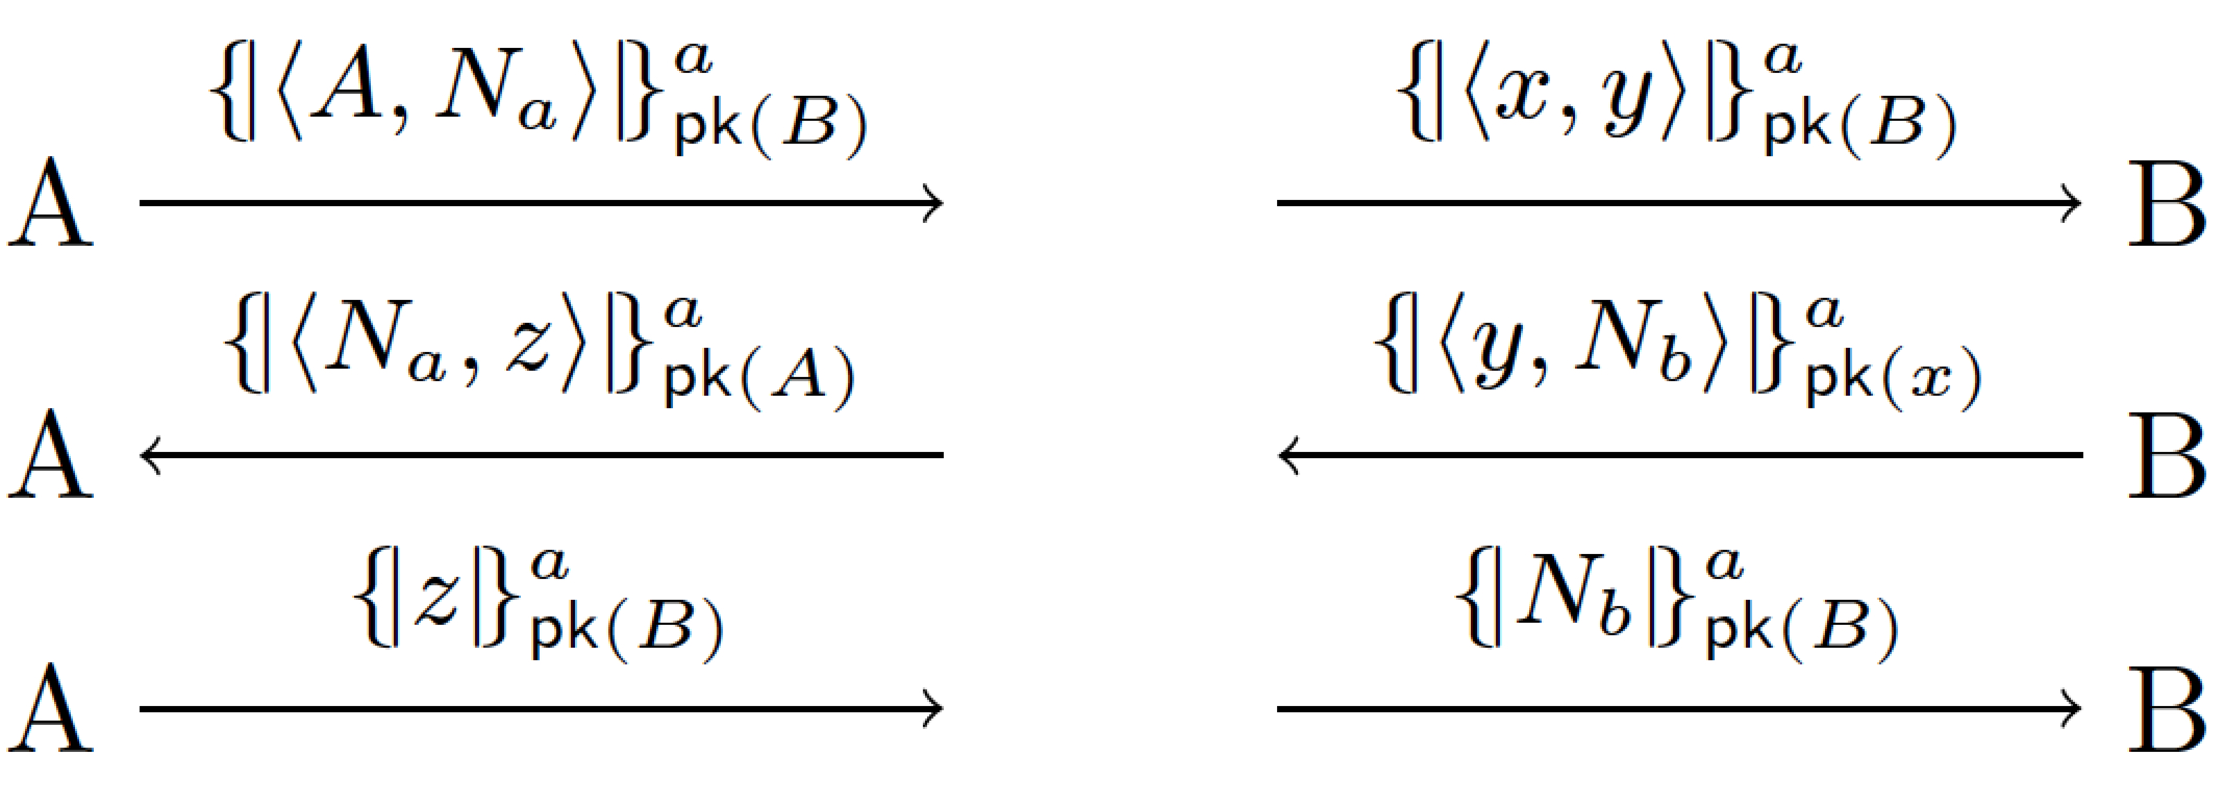
\includegraphics[width=0.6\textwidth, angle=0]{Graphics/NS_Protocol.pdf}
\end{center}

The A and B each represent Alice and Bob, while the arrows indicates the direction of the sent and received messages, by which are illustrated above each line. The notation $\{| m |\}^a_{pk(B)}$ denotes that the message \textit{m} is created with an asymmetric encryption of Bob's public key, while the $\langle m_1, m_2 \rangle$ illustrates a pairing, so a concatenation of the two messages. \textit{A} and \textit{B} in the messages, each represent the identities of Alice and Bob, while \textit{N$_a$} denotes the freshly generated nonce, a random number generated each session. The variables \textit{x, y, z} are used for the unknown values of the message.

In the first exchange, Alice sends her identity and nonce asymmetrically encrypted with Bob's public key. Bob receives the message, with variables \textit{x, y} illustrating the unknown values of the message. Bob decrypts the message, to check that it is well-formed. He then generate his own nonce, pair it with Alice's nonce, and then encrypts it with Alice's public key. Alice then decrypts Bob's message, to verify that it contains her previously sent nonce, which proves that Bob received her first message. 
This way of sending and receiving nonces is often called a \textit{challenge-response} authentication \autocite{DBLP:journals/ftpl/CortierK14}, and is also what you see when using passwords, where the challenger asks for a password and then checks that the response is valid. 
\bigbreak
The gap left between the two participants illustrate the challenge of this protocol in an untrusted network, as an attacker may instigate a man-in-the-middle attack. This vulnerability of the protocol, was first described by Gavin Lowe in his paper published in 1995, where a fix was also purposed. Again the Alice and Bob notation is used, but now we introduce an adversary \textit{C}, as illustrated here by \citeauthor{DBLP:journals/ftpl/CortierK14}.

\begin{center}
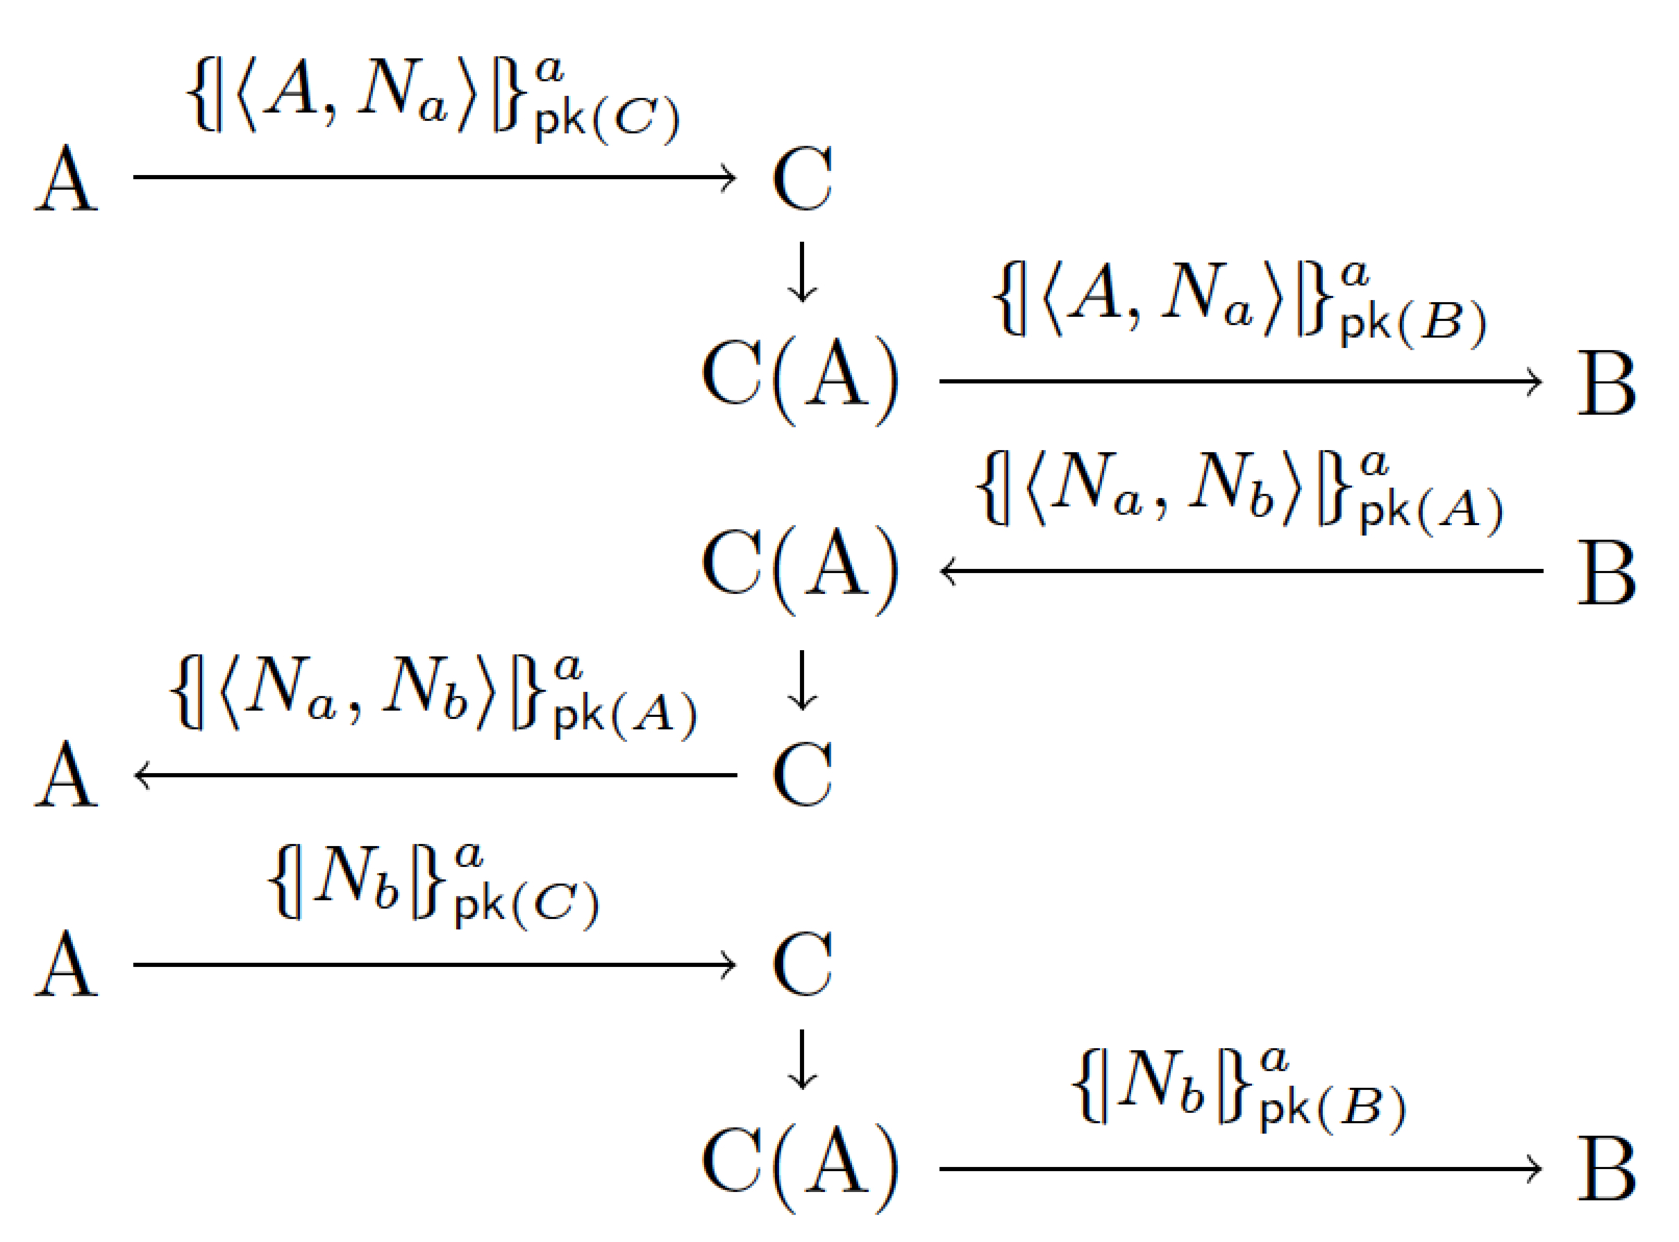
\includegraphics[width=0.55\textwidth, angle=0]{Graphics/Challenge.pdf}
\end{center}

If the attacker can persuade \textit{A} to initiate a session with him, he relay the messages to \textit{B}, and thus convince him he is communicating with \textit{A}. Lowe suggest a simple solution to this problem, by adding the identity of the sender in the second message so that $\{|\langle N_a, N_b\rangle |\}^a_{pk(a)}$ would now look as such $\{|\langle N_a, \langle N_b, B\rangle \rangle |\}^a_{pk(a)}$


\iffalse
A -> B : m  			= Alice sends Bob a message
Notation {|m|}^a_pk(B) 	= asymmetric encryption of m with Bob's public key. 
<m1, m2>				= pairing, i.e. concatenation of the two messages
A, B					= Their identities
N_a					= nonce (number used once - fresh random generated each session)
x, y, z				= Variables for unknown component(values)

First 					= Alice sends her identity and nonce, encrypted with Bob's public key

Bob then decrypts and check that it is well-formed.
This mechanism of sending someone an encrypted nonce and waiting for the recipient to send back this nonce is often called a challenge-response mechanism.
Alice then decrypts Bob's message, and verifies that it contains har previous N_a - proves that Bob received first message

The aim of the protocol is to guarantee mutual 'authentication' - ensures they have been communicating with the right person
Moreover, the protocol should guarantee 'confidentiality' of the nonces Na and Nb.
 - Honest execution (man in the middle attack)
\fi

\subsection{Message deduction}
Message deduction is a formal way of figuring out wether a message can be deducted from a priori given set of messages through induction rules and derivation sequences. This \\ \\
\textbf{TODO: Terms} \\ \\
\textbf{Inference rules(system)} \\
%TODO: Introduce the Dolev-Yao model from 1981 - first symbolic formalisation of the deductive power of an attacker
Inference rules uses the following notation $\infer{u} {u_l & ... & u_n}$ with $u_l,...,u_n, u$ as terms with variables. Having a set of inference rules is also called an inference system, and often contains both \textit{composition rules} and \textit{decomposition rules}. Below can be seen an inference system for the Dolev-Yao model ($\mathcal{I}_{DY}$) with the composition rules presented first in each line, and the rest being the decomposition rules. 
\begin{center}
$\mathcal{I}_{DY}\ :$
\begin{math}
  \left\{
    \begin{array}{l l l}
      \infer{\langle x, y \rangle}{x,y} \qquad \infer{x}{\langle x, y \rangle} \qquad \infer{y}{\langle x, y \rangle} \\ \\
      \infer{\text{senc}(x, y)}{x\ y} \qquad  \infer{x}{\text{senc}(x, y)\ y} \\ \\
      \infer{\text{aenc}(x, y)}{x\ y} \qquad \infer{x}{\text{aenc}(x, \text{pk}(y))\ y}
    \end{array}
  \right.
\end{math}
\end{center}
\bigbreak
\noindent First line - anyone can concatenate terms and retrieve terms from a concatenation. \\
Second line - one can encrypt and decrypt symmetrically whenever he has the corresponding key \\
Third line - same as two, but with asymmetric encryptions 

\textbf{TODO: Derivation sequence (Deduction rules?)} \\
Inference rules can be combined to compute or derive new messages (rewrite). 
 

%\subsection{Examples}
%TODO: show examples of a man in the middle attack on the NS and DH protocols: \\ \\
%- Needham-Schroeder Public key protocol (now modified according to Lowe's man in the middle attack): 


